\documentclass[12pt,a4paper]{article}

% --- Pacotes essenciais de formatação ---
\usepackage[utf8]{inputenc}
\usepackage[T1]{fontenc}
\usepackage[brazil]{babel}
\usepackage{mathptmx} % Fonte Times New Roman estrita (igual ao modelo)
\usepackage[left=3.0cm, top=3.0cm, right=2.0cm, bottom=2.0cm]{geometry}
\usepackage{setspace}
\onehalfspacing % Espaçamento 1.5 entre linhas

\usepackage{indentfirst}
\setlength{\parindent}{1.25cm} % Recuo padrão de parágrafo ABNT
\setlength{\parskip}{0pt}

\usepackage{graphicx}
\graphicspath{{prints/}}
\usepackage{xcolor}
\usepackage{amsmath,amssymb}
\usepackage{listings}
\usepackage{fancyhdr}
\usepackage{titlesec}
\usepackage{caption}
\usepackage{tabularx}
\usepackage{array}
\usepackage{float}
\usepackage{hyperref}
\usepackage[htt]{hyphenat}
\usepackage{microtype}

% Permite quebra suave de linha em identificadores com sublinhado em texto e \texttt
\renewcommand{\_}{\textunderscore\allowbreak}

% Otimizacao do posicionamento de figuras para evitar paginas vazias
\renewcommand{\topfraction}{0.85}
\renewcommand{\bottomfraction}{0.85}
\renewcommand{\textfraction}{0.15}
\renewcommand{\floatpagefraction}{0.70}

\raggedbottom % Impede o esticamento vertical de paginas evitando grandes vazios brancos
\sloppy       % Evita estouro de palavras longas e codigo na margem direita

% --- Configuração de Cabeçalho e Rodapé (Número da página no canto inferior direito) ---
\pagestyle{fancy}
\fancyhf{}
\fancyfoot[R]{\thepage}
\renewcommand{\headrulewidth}{0pt}
\renewcommand{\footrulewidth}{0pt}

% --- Configuração estrita de Títulos de Seção (igual ao modelo: 1. Introdução, etc.) ---
\titleformat{\section}
  {\normalfont\bfseries\normalsize}
  {\thesection.}
  {0.5em}
  {}

\titleformat{\subsection}
  {\normalfont\bfseries\normalsize}
  {\thesubsection}
  {0.5em}
  {}

\titleformat{\subsubsection}
  {\normalfont\bfseries\normalsize}
  {\thesubsubsection}
  {0.5em}
  {}

\titlespacing*{\section}{0pt}{1.5ex plus 0.5ex minus 0.2ex}{0.8ex plus 0.2ex}
\titlespacing*{\subsection}{0pt}{1.2ex plus 0.4ex minus 0.2ex}{0.6ex plus 0.2ex}
\titlespacing*{\subsubsection}{0pt}{1.0ex plus 0.3ex minus 0.2ex}{0.5ex plus 0.2ex}

% --- Formatação de Legenda das Figuras (Ex: Figura 1- Nome da figura em negrito e centralizado) ---
\DeclareCaptionLabelSeparator{hifen}{-- }
\captionsetup[figure]{
    name=Figura,
    labelsep=hifen,
    justification=centering,
    font=bf,
    labelfont=bf
}

% --- Configuração de Links ---
\hypersetup{
    colorlinks=true,
    linkcolor=black,
    citecolor=blue,
    urlcolor=blue
}

% --- Configuração do Listings para Código em C ---
\definecolor{codegreen}{rgb}{0,0.5,0}
\definecolor{codegray}{rgb}{0.45,0.45,0.45}
\definecolor{codepurple}{rgb}{0.55,0,0.75}
\definecolor{backcolour}{rgb}{0.98,0.98,0.98}

\lstdefinestyle{estiloc}{
    backgroundcolor=\color{backcolour},
    commentstyle=\color{codegreen}\itshape,
    keywordstyle=\color{blue}\bfseries,
    numberstyle=\tiny\color{codegray},
    stringstyle=\color{codepurple},
    basicstyle=\ttfamily\footnotesize,
    breakatwhitespace=false,
    breaklines=true,
    captionpos=b,
    keepspaces=true,
    numbers=left,
    numbersep=6pt,
    showspaces=false,
    showstringspaces=false,
    showtabs=false,
    tabsize=2,
    frame=single,
    rulecolor=\color{black!25}
}
\lstset{style=estiloc}

\begin{document}

% =========================================================================
% CAPA (Idêntica à Página 1 do modelo de referência da UFV Florestal)
% =========================================================================
\thispagestyle{empty}
\begin{center}
    % Logo UFV estilizado em vetor / texto com as cores oficiais (dispensa dependência de arquivo externo)
    {\fontsize{38}{42}\selectfont \textbf{\textsf{\textcolor[RGB]{25,25,25}{U}\hspace{1pt}\textcolor[RGB]{150,20,20}{F}\hspace{1pt}\textcolor[RGB]{200,140,20}{V}}}}\\[0.25cm]
    {\normalsize SERVIÇO PÚBLICO FEDERAL $\cdot$ MINISTÉRIO DA EDUCAÇÃO}\\[0.12cm]
    {\normalsize UNIVERSIDADE FEDERAL DE VIÇOSA $\cdot$ UFV}\\[0.12cm]
    {\normalsize CAMPUS FLORESTAL}\\[4.8cm]

    {\large \textbf{Trabalho 1 - PAA}}\\[0.3cm]
    {\large \textbf{Resolução de Labirinto com Backtracking}}\\[5.0cm]

    \begin{flushright}
        Gabriel Marcus de Oliveira Felix --- Matrícula: 5792 \\
        Otávio Soares Pedroso --- Matrícula: 6593 \\
        Pedro Mendes Gonzaga --- Matrícula: 6563 \\
        Rafaella Ferreira Pinheiro Silva --- Matrícula: 5363 \\
        Tomás Viana Resende --- Matrícula: 6556
    \end{flushright}

    \vfill
    {\normalsize Florestal - MG}\\[0.12cm]
    {\normalsize 2026}
\end{center}

% =========================================================================
% SUMÁRIO (Idêntico à Página 2 do modelo de referência)
% =========================================================================
\newpage
\setcounter{page}{2}
\thispagestyle{fancy}

\begin{center}
    \textbf{\large Sumário}
\end{center}
\vspace{1.0cm}

\noindent
Sumário \hfill 2\\[0.35cm]
\textbf{1. Introdução} \hfill 3\\[0.35cm]
\textbf{2. Organização} \hfill 3\\[0.35cm]
\textbf{3. Desenvolvimento} \hfill 4\\[0.35cm]
\textbf{4. Resultados} \hfill 6\\[0.35cm]
\textbf{5. Conclusão} \hfill 9\\[0.35cm]
\textbf{6. Referências} \hfill 9

% =========================================================================
% 1. INTRODUÇÃO (Idêntico à Página 3 do modelo de referência)
% =========================================================================
\newpage
\section{Introdução}

Esta documentação se refere ao projeto feito no Trabalho Prático 1, da disciplina PROJETO E ANÁLISE DE ALGORITMOS, ministrada na Universidade Federal de Viçosa (UFV) -- Campus Florestal. No trabalho, foi proposta a implementação de um programa em linguagem C para a resolução exaustiva de um problema de exploração de labirintos pautado no paradigma de \textbf{Backtracking}, visando determinar a existência de uma rota viável entre a posição inicial do aventureiro e a câmara que abriga um baú de tesouros, e a montagem de tabelas e gráficos para analisar seu tempo de execução, a fim de aprender sobre complexidade de algoritmos. O projeto descrito neste documento está versionado e documentado no repositório oficial do grupo.

O labirinto bidimensional impõe restrições essenciais ao aventureiro:
\begin{itemize}
    \item Cada sala (célula da matriz) pode ser visitada no máximo uma única vez durante a trajetória, impedindo a ocorrência de ciclos;
    \item O baú misterioso somente pode ser destrancado caso o aventureiro colete a quantidade exata de chaves exigida;
    \item Apenas movimentos cardeais ortogonais são admitidos (Cima, Baixo, Esquerda e Direita), sendo vedados saltos ou diagonais;
    \item Paredes intransponíveis não podem ser atravessadas.
\end{itemize}

Foram utilizadas as bibliotecas padrão da linguagem C: “stdio.h”, “stdlib.h”, “string.h”, “time.h” e “unistd.h”. A biblioteca “time.h” foi utilizada para calcular a duração das execuções no benchmark, “stdlib.h” para gerenciamento de memória e números aleatórios no gerador, “stdio.h” para entrada e saída de arquivos, “string.h” para argumentos de linha de comando, e “unistd.h” para o controle de temporização da animação no terminal. O programa foi estruturado em módulos independentes, separando o algoritmo de busca, as regras de navegação, a interface de usuário e a infraestrutura de medição de desempenho.

% =========================================================================
% 2. ORGANIZAÇÃO (Idêntico à Página 3 e 4 do modelo)
% =========================================================================
\section{Organização}

Na pasta principal do repositório podem ser encontrados os diretórios e arquivos do projeto, com os seguintes nomes: \texttt{src} (pasta com os códigos-fonte C), \texttt{include} (pasta com os cabeçalhos \texttt{.h}), \texttt{docs} (pasta com a documentação técnica e relatório em \LaTeX), \texttt{entradas} (pasta com os arquivos de labirinto em formato texto \texttt{.txt}), \texttt{Makefile} e \texttt{README.md}.

Em \texttt{entradas} encontram-se as instâncias de teste do labirinto: “trivial.txt”, “exemplo.txt” e “grande.txt”. Já na pasta \texttt{src} temos os seguintes módulos: “mapa.c”, “gerador.c”, “backtracking.c”, “navegacao.c”, “cli.c”, “analise.c”, “visualizador.c”, “saida.c”, “benchmark.c” e “main.c”. Na pasta \texttt{include} encontram-se as respectivas interfaces: “mapa.h”, “backtracking.h”, “navegacao.h”, “cli.h”, “analise.h”, “visualizador.h” e “saida.h”.

\begin{figure}[htbp]
    \centering
    \begin{minipage}{0.7\textwidth}
        \ttfamily\small
        \begin{tabular}{|l|}
        \hline
        PAA\_TP01/ \\
        \quad |-- docs/ (relatorio.tex, capitulos em markdown) \\
        \quad |-- entradas/ (trivial.txt, exemplo.txt, grande.txt) \\
        \quad |-- include/ (mapa.h, backtracking.h, navegacao.h, cli.h, ...) \\
        \quad |-- src/ (main.c, mapa.c, backtracking.c, navegacao.c, ...) \\
        \quad |-- Makefile \\
        \quad |-- README.md \\
        \hline
        \end{tabular}
    \end{minipage}
    \vspace{0.2cm}
    \caption{Repositório do projeto}
\end{figure}

Sendo assim, a pasta principal do projeto contém arquivos referentes ao repositório do Git, e as subpastas contendo os códigos, além de arquivos referentes à especificação do trabalho prático e ao Makefile para automação de compilação sem advertências (\textit{warnings}).

% =========================================================================
% 3. DESENVOLVIMENTO (Idêntico às Páginas 4 e 5 do modelo)
% =========================================================================
\section{Desenvolvimento}

\subsection{“mapa.c”, “mapa.h” e “gerador.c”}

O módulo do mapa é responsável pelo gerenciamento estrutural dos dados do labirinto, pelo carregamento e validação de arquivos de texto, pelo controle seguro de memória dinâmica na \textit{Heap} e pela implementação do programa independente gerador de mapas (\textbf{Extra 1}).

No cabeçalho \texttt{mapa.h} foram concebidas as estruturas de dados fundamentais:
\begin{itemize}
    \item \texttt{TipoCelula}: tipo enumerado que define semanticamente cada sala da matriz (\texttt{SALA\_VAZIA}, \texttt{PAREDE}, \texttt{CHAVE}, \texttt{BAU} e \texttt{AVENTUREIRO}), propiciando clareza semântica e segurança de tipos;
    \item \texttt{Labirinto}: registro principal que agrega as dimensões da grade (linhas e colunas), o total de chaves requeridas, os pontos de partida e do baú pré-indexados, além do ponteiro duplo para a matriz (\texttt{TipoCelula **grade});
    \item \texttt{Posicao} e \texttt{Caminho}: estrutura dinâmica de coordenadas para registro do trajeto. Sua capacidade expande geometricamente via \texttt{realloc}, assegurando custo amortizado $\mathcal{O}(1)$ por inserção.
\end{itemize}

\textbf{“carregar\_labirinto”}: Abre o arquivo texto, lê e valida as dimensões e o total de chaves com \texttt{fscanf}, aloca a matriz bidimensional e mapeia os tokens para \texttt{TipoCelula}. Valida a existência de exatamente um ponto de partida \texttt{A} e um baú \texttt{X}. Caso ocorra qualquer erro de alocação ou dados corrompidos, a função realiza a desalocação em cascata de todas as linhas alocadas anteriormente antes de retornar \texttt{NULL}, garantindo falha segura.

\textbf{“liberar\_labirinto”}: Desaloca linha por linha a matriz de células, o vetor de ponteiros e a struct raiz, eliminando qualquer possibilidade de vazamento de memória (\textit{memory leak}).

A alocação matricial na \textit{Heap} e a hierarquia de ponteiros do labirinto são ilustradas esquematicamente na Figura~\ref{fig:diagrama_memoria}:

\begin{figure}[htbp]
    \centering
    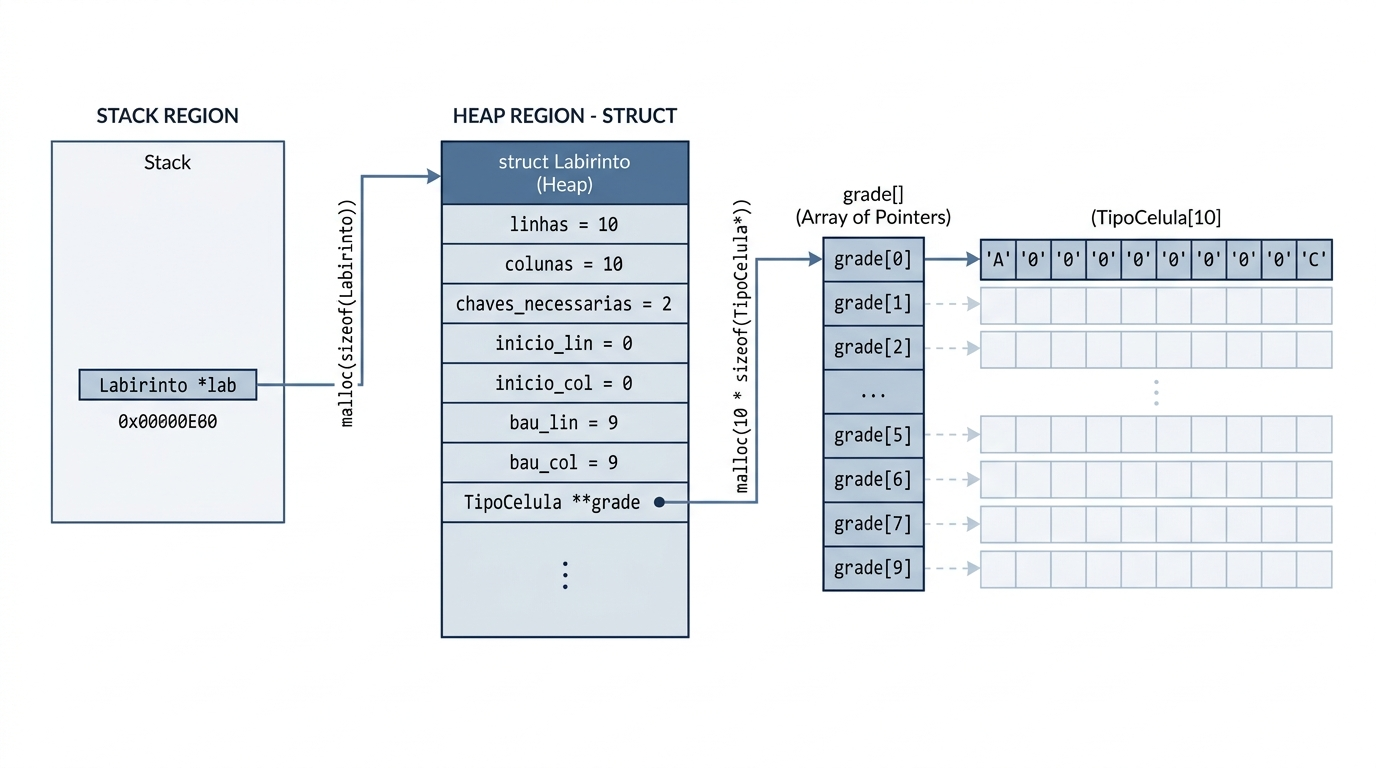
\includegraphics[width=0.58\textwidth]{prints/diagrama_memoria.png}
    \vspace{0.15cm}
    \caption{Diagrama esquemático da alocação de memória do Labirinto na Heap}
    \label{fig:diagrama_memoria}
\end{figure}

\subsubsection*{Gerador de Mapas Solúveis (gerador.c — Extra 1)}

Para atender ao \textbf{Extra 1}, foi desenvolvido o programa independente \texttt{gerador.c}. Sorteios puramente aleatórios de células com probabilidade estática frequentemente geram labirintos desconexos ou com chaves isoladas por paredes, tornando-os insolúveis. Para contornar esse problema e viabilizar testes rigorosos, o gerador adota uma abordagem construtiva garantida:
\begin{enumerate}
    \item \textbf{Caminho Garantido via DFS Randomizada}: A partir de $A$ em $(0,0)$, executa-se uma Busca em Profundidade traçando uma rota sinuosa e sem repetições até o baú em $(linhas-1, colunas-1)$. Caso a busca sempre tentasse as direções na mesma ordem fixa (ex.: sempre Cima antes de Baixo), todos os mapas gerados teriam trajetórias repetitivas e com o mesmo padrão geométrico. Para garantir caminhos orgânicos e imprevisíveis a cada geração, a função auxiliar \texttt{embaralhar} aplica a permutação de Fisher-Yates, que sorteia uniformemente a ordem das 4 direções a cada passo da busca, conforme ilustrado na Figura~\ref{fig:dfs_gerador};
    \item \textbf{Distribuição Protegida das Chaves}: As células do caminho encontrado são marcadas em uma máscara de proteção. As chaves exigidas são sorteadas exclusivamente entre as posições intermediárias dessa rota garantida, assegurando matematicamente que o aventureiro poderá alcançá-las;
    \item \textbf{Inserção de Paredes}: As células externas ao caminho protegido recebem paredes com probabilidade parametrizável (padrão de 35\%), preservando a existência de ao menos uma solução viável.
\end{enumerate}

\begin{figure}[htbp]
    \centering
    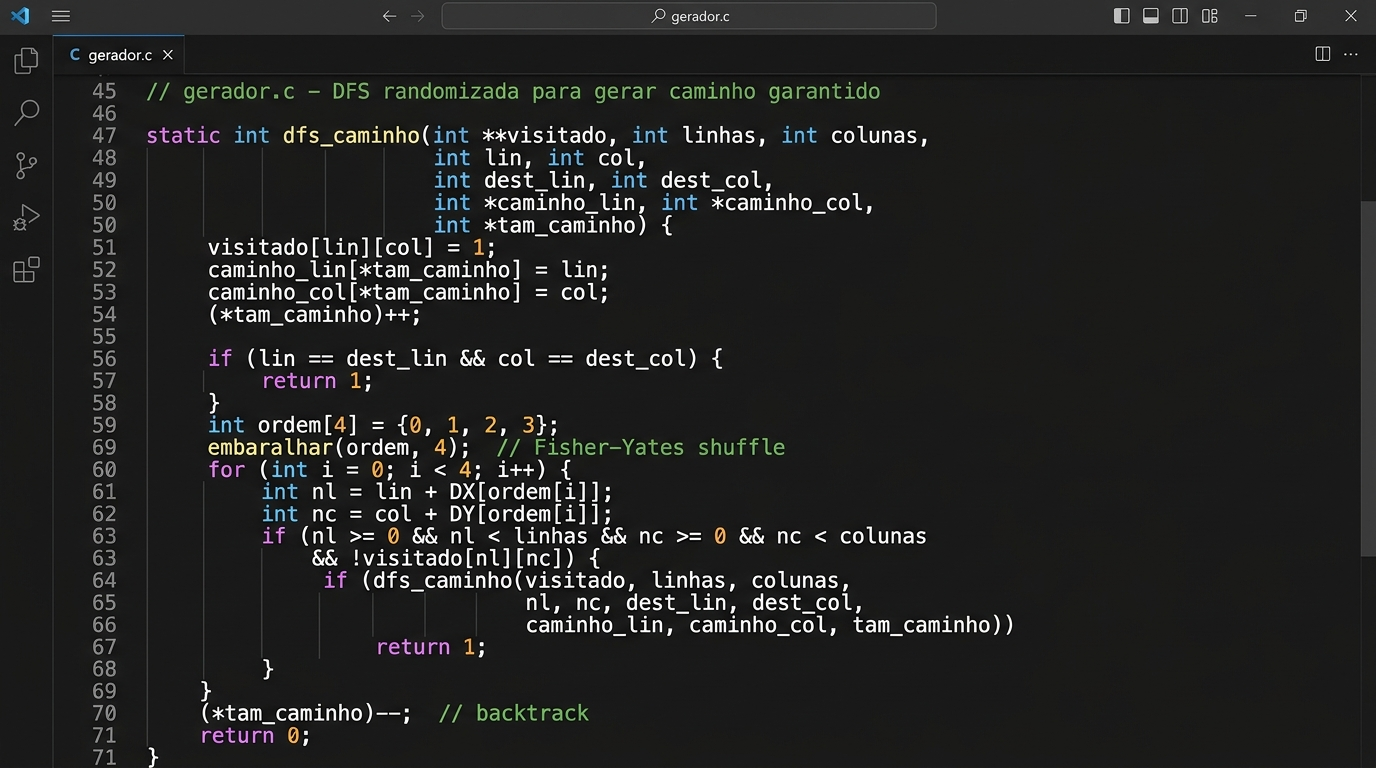
\includegraphics[width=0.70\textwidth]{prints/dfs_gerador.png}
    \vspace{0.15cm}
    \caption{Implementação do embaralhamento de direções com Fisher-Yates no gerador}
    \label{fig:dfs_gerador}
\end{figure}

O gerador é invocado via linha de comando recebendo os parâmetros de dimensão e regras:
\begin{center}
\small
\texttt{./bin/gerador <linhas> <colunas> <num\_chaves> <saida.txt> [seed] [prob]}
\end{center}
O suporte a semente (\texttt{seed}) permite reproduzir os mesmos cenários para fins de comparação empírica no \textit{benchmark}. A compilação e a execução do gerador no terminal são demonstradas na Figura~\ref{fig:terminal_gerador}:

\begin{figure}[htbp]
    \centering
    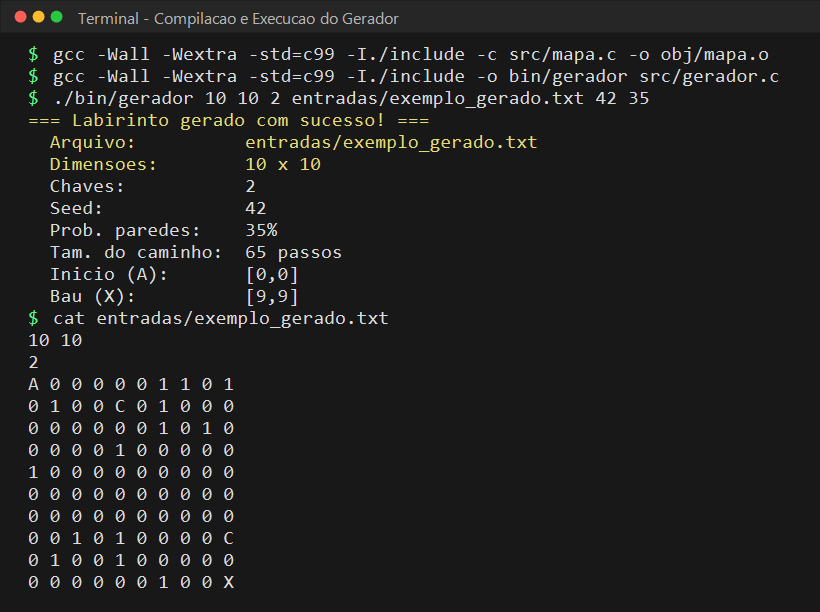
\includegraphics[width=0.70\textwidth]{prints/terminal_compilacao.png}
    \vspace{0.15cm}
    \caption{Compilação sem advertências e execução do gerador via linha de comando}
    \label{fig:terminal_gerador}
\end{figure}

\subsection{“backtracking.c” e “backtracking.h”}
Nestes arquivos foi desenvolvido o núcleo algorítmico do trabalho: um motor de busca em profundidade com retrocesso sistemático (\textit{backtracking}) e podas por inviabilidade. O algoritmo atua como integrador dos módulos descritos anteriormente: consome a matriz e o vetor dinâmico de coordenadas de \texttt{mapa.h}, delega a validação geométrica de passos a \texttt{navegacao.h} e registra métricas na estrutura de \texttt{analise.h}.

A função de entrada \textbf{“resolver\_labirinto\_completo”} prepara o ambiente antes de iniciar a exploração:
\begin{enumerate}
    \item Aloca dinamicamente a matriz bidimensional de visitados (\texttt{visitado}) utilizando a função utilitária \texttt{alocar\_matriz\_int} de \texttt{mapa.c};
    \item Inicializa a estrutura de caminho temporário (\texttt{caminho\_init});
    \item Caso a flag \texttt{--analise} esteja ativa, dispara \texttt{analise\_iniciar} para zerar contadores de chamadas, podas e profundidade;
    \item Invoca a rotina recursiva \textbf{“backtrack\_recursivo”} a partir da coordenada inicial do aventureiro (\texttt{inicio\_lin}, \texttt{inicio\_col}), com contagem inicial de 0 chaves e profundidade 1;
    \item Ao término da busca, desaloca a matriz de visitados (\texttt{liberar\_matriz\_int}) e o caminho temporário, garantindo ausência de vazamentos de memória.
\end{enumerate}

Para cada célula navegada, a função recursiva delega o cálculo das coordenadas vizinhas e a checagem de barreiras às funções \texttt{proxima\_posicao} no modo padrão, ou \texttt{proxima\_posicao\_globo} caso a navegação toroidal esteja ativa. Caso o movimento seja inválido (ao atingir uma parede ou uma célula já visitada), o algoritmo computa uma poda (\texttt{analise\_registrar\_poda}) e não aprofunda a chamada.

\begin{lstlisting}[language=C, caption={Trecho central de exploração recursiva e gestão de chaves no backtracking.}]
/* Fazer a escolha: visitar a celula */
visitado[lin][col] = 1;
caminho_adicionar(caminho_atual, lin, col);

int pegou_chave = 0;
if (lab->grade[lin][col] == CHAVE) {
    chaves_coletadas++;
    pegou_chave = 1;
}

/* Caso Base e Poda do Bau */
if (lab->grade[lin][col] == BAU) {
    if (chaves_coletadas == lab->chaves_necessarias) {
        /* Solucao viavel encontrada! */
        return 1;
    } else {
        /* Poda: atingir o bau sem todas as chaves e um beco sem saida definitivo */
        caminho_remover_ultimo(caminho_atual);
        visitado[lin][col] = 0;
        return 0;
    }
}
\end{lstlisting}

\textbf{Decisões de Implementação e Dificuldades Superadas:}
\begin{enumerate}
    \item \textbf{Gestão Reversível do Contador de Chaves:} Um dos desafios críticos em problemas combinatórios reside em garantir a integridade do estado ao retroceder na árvore de busca. Caso uma sala visitada contenha uma chave (\texttt{CHAVE}), o contador é incrementado e a variável local \texttt{pegou\_chave} é assinalada como verdadeira. Ao término da exploração de todas as ramificações filhas, se a busca precisar retroceder (\textit{backtrack}), a condição \texttt{if (pegou\_chave) chaves\_coletadas--;} desfaz a alteração, garantindo que nenhum caminho alternativo herde chaves coletadas em ramos descartados.
    \item \textbf{Poda por Inviabilidade Futura no Baú e Ganho de Complexidade:} O regulamento proíbe estritamente passar pela mesma sala mais de uma vez (ausência de ciclos). Logo, caso o aventureiro ingresse na sala do baú (\texttt{BAU}) sem todas as chaves, essa rota torna-se matematicamente sem saída: se continuasse explorando a partir dali, o baú ficaria bloqueado como visitado e o aventureiro jamais conseguiria retornar a ele para destrancá-lo. Em vez de gastar recursão desnecessária, o algoritmo realiza uma **poda imediata** (\textit{pruning}) retornando falha. Essa decisão corta na raiz subárvores de profundidade que poderiam alcançar até $L \times C$ passos, reduzindo o fator de ramificação efetivo da busca e diminuindo drasticamente a quantidade de chamadas recursivas e o tempo prático de resolução.
    \item \textbf{Busca Exaustiva e Cópia Profunda de Múltiplos Caminhos (Extra 2):} No modo padrão, a exploração encerra-se na primeira rota válida encontrada. O \textbf{Extra 2} (\texttt{--todos}) introduz a busca exaustiva por todas as soluções possíveis. Como o vetor dinâmico de coordenadas (\texttt{caminho\_atual}) sofre sucessivos retrocessos (via rotina \texttt{caminho\_remover\_ultimo}) para testar alternativas distintas, salvar apenas ponteiros faria com que todas as rotas armazenadas ficassem corrompidas ou vazias no final. Para contornar essa restrição da linguagem C, implementou-se a função \texttt{caminho\_copiar}, que realiza uma cópia profunda (\textit{deep copy}): aloca um novo bloco na memória \textit{Heap} e duplica todas as coordenadas da rota encontrada. Esse trajeto clonado é armazenado na estrutura dinâmica \texttt{ListaCaminhos}, que expande sua capacidade geometricamente sob demanda. Após registrar a solução, o algoritmo desmarca a sala e força o retrocesso programado para continuar explorando o labirinto até esgotar todas as combinações viáveis, permitindo ao final relatar o total de rotas e imprimi-las individualmente.
\end{enumerate}

\subsection{“navegacao.c” e “cli.c”}

Este módulo é responsável por isolar duas tarefas essenciais do projeto: o controle das regras de movimentação física do aventureiro sobre a grade e a interpretação dos comandos passados pelo usuário no terminal.

\subsubsection*{1. Regras de Movimentação e Modo Globo (navegacao.c)}

O aventureiro só pode se deslocar nas quatro direções cardeais ortogonais (Cima, Baixo, Esquerda e Direita). Para simplificar o laço de repetição do \textit{backtracking} e evitar estruturas condicionais repetitivas, as transições foram organizadas em dois vetores estáticos constantes:
\begin{lstlisting}[language=C, caption={Vetores de deslocamento ortogonal em O(1).}]
const int DIRECOES_LIN[NUM_DIRECOES] = {-1,  1,  0,  0};
const int DIRECOES_COL[NUM_DIRECOES] = { 0,  0, -1,  1};
\end{lstlisting}

A função \textbf{“movimento\_valido”} verifica se a próxima sala pode ser acessada, aplicando as restrições obrigatórias:
\begin{enumerate}
    \item Estar dentro das dimensões da grade ($0 \le lin < linhas$ e $0 \le col < colunas$);
    \item Não ser uma parede intransponível (\texttt{grade[lin][col] != PAREDE});
    \item Não ter sido visitada no caminho atual (\texttt{visitado[lin][col] == 0}).
\end{enumerate}

\textbf{Ordem das validações:} A checagem de limites é feita antes do acesso à matriz de células. Graças à avaliação em curto-circuito da linguagem C, se a coordenada estiver fora do mapa, a função retorna zero imediatamente sem acessar posições de memória ilegais, evitando erros de segmentação (\textit{segmentation fault}).

Para o \textbf{Modo Globo (Extra 3)}, o mapa funciona de forma toroidal (semelhante ao clássico jogo da cobrinha): ao ultrapassar uma borda, o personagem reaparece no lado oposto do labirinto. Essa transição circular é calculada diretamente com o operador de resto da divisão:
\begin{lstlisting}[language=C, caption={Cálculo da próxima posição com conexão toroidal das bordas.}]
*prox_lin = (lin + DIRECOES_LIN[d] + lab->linhas)  % lab->linhas;
*prox_col = (col + DIRECOES_COL[d] + lab->colunas) % lab->colunas;
\end{lstlisting}
Somar o total de linhas e colunas antes da operação de resto é fundamental para garantir que coordenadas negativas (como tentar subir a partir da linha 0) não gerem números negativos em C, resultando sempre no índice correto da borda oposta.

\subsubsection*{2. Interface de Linha de Comando (cli.c)}

O módulo de CLI permite ao usuário configurar a execução através de flags no terminal sem alterar o código. Todas as opções são concentradas na estrutura \texttt{Opcoes}:
\begin{lstlisting}[language=C, caption={Estrutura de dados Opcoes para controle de parâmetros e flags.}]
typedef struct {
    const char *arquivo_entrada; /* Caminho do arquivo .txt do labirinto */
    int modo_globo;              /* 1: movimentacao toroidal (--globo) */
    int modo_todos;              /* 1: busca exaustiva de todos os caminhos (--todos) */
    int modo_analise;            /* 1: exibicao de nos e profundidade (--analise) */
    int modo_visual;             /* 1: animacao colorida ANSI no terminal (--visual) */
} Opcoes;
\end{lstlisting}

A função \textbf{“cli\_parse”} varre os argumentos do terminal (\texttt{argv}): argumentos iniciados por \texttt{--} ativam as flags correspondentes, enquanto o argumento sem prefixo é identificado como o arquivo de entrada. Se nenhum arquivo for informado, o programa exibe automaticamente as instruções de uso (\textbf{“cli\_usage”}) com todos os comandos aceitos e encerra a execução de forma segura.

\subsection{“analise.c” e “visualizador.c”}
Nestes arquivos foi implementada a instrumentação de desempenho computacional e a interface visual interativa em terminal:

\textbf{“analise\_registrar\_chamada”}: Contabiliza a quantidade de nós visitados e a profundidade máxima alcançada pela pilha de recursão.

\textbf{“visualizar\_passo”}: Utiliza sequências de escape ANSI para colorir e atualizar a grade do labirinto no terminal quadro a quadro, conferindo efeito de animação da busca.

\subsection{“saida.c”, “benchmark.c” e “main.c”}
\textbf{“imprime\_caminho”}: Formata a rota percorrida no padrão exigido pela especificação: $[l_1,c_1],[l_2,c_2],\dots,[l_k,c_k]$.

\textbf{“executa\_benchmark”}: Realiza baterias de testes temporizadas com a biblioteca \texttt{time.h}, permitindo avaliar a curva de crescimento do tempo computacional.

\textbf{“main”}: Atua como orquestrador central de todo o fluxo de processamento, integrando de forma desacoplada os módulos de leitura de mapa, análise de linha de comando, motor de busca recursivo, medição de tempo e saída de resultados.

\textbf{Decisão de Projeto (Modularização e Encapsulamento da Linha de Comando):} No projeto inicial, a validação de parâmetros era efetuada de maneira elementar no próprio corpo da função \texttt{main} por meio da condicional \texttt{if (argc < 2)}, assumindo-se rigidamente que o arquivo de labirinto estaria na posição \texttt{argv[1]}. Contudo, com a introdução das flags dos modos operacionais (\texttt{--globo}, \texttt{--todos}, \texttt{--analise} e \texttt{--visual}), essa checagem ingênua tornou-se insuficiente e sujeita a falhas caso as opções fossem fornecidas antes do nome do arquivo. Como decisão de engenharia de software e visando à estrita modularização exigida na disciplina, toda a análise sintática de argumentos e tratamento de erro de entrada foram delegados à função \texttt{cli\_parse} do módulo \texttt{cli.c}. Assim, o \texttt{main} permanece enxuto e coeso, operando apenas com a estrutura unificada \texttt{Opcoes}, em conformidade com o princípio de responsabilidade única.

% =========================================================================
% 4. RESULTADOS (Idêntico às Páginas 6, 7 e 8 do modelo)
% =========================================================================
\newpage
\section{Resultados}

\subsection{Exemplo de Execução no Modo Padrão}

O programa implementado conta com interface de linha de comando para que o usuário informe o arquivo de teste desejado e selecione as opções de resolução. Caso o usuário não informe um arquivo existente ou omita parâmetros essenciais, o sistema trata o erro amigavelmente:

\begin{figure}[htbp]
    \centering
    \begin{minipage}{0.75\textwidth}
        \ttfamily\small
        \begin{tabular}{|l|}
        \hline
        \$ ./bin/labirinto \\
        Erro: nenhum arquivo de labirinto informado. \\[0.2cm]
        Uso: ./bin/labirinto <arquivo\_labirinto.txt> [opcoes] \\
        Opcoes: \\
        \quad --globo    Ativa modo globo (labirinto toroidal, bordas se conectam) \\
        \quad --todos    Encontra e exibe todos os caminhos possiveis ate o bau \\
        \quad --analise  Exibe metricas de recursao (chamadas totais e nivel maximo) \\
        \quad --visual   Visualizador ANSI: imprime o labirinto colorido no terminal \\
        \hline
        \end{tabular}
    \end{minipage}
    \vspace{0.2cm}
    \caption{Tratamento de erro e exibição de ajuda amigável pelo módulo CLI}
    \label{fig:erro_cli}
\end{figure}

Ao fornecer um labirinto válido juntamente com a opção \texttt{--analise}, o programa calcula a rota, formata as coordenadas no padrão exigido e exibe o sumário estatístico gerado pela instrumentação de recursão, como demonstrado na Figura~\ref{fig:execucao_padrao}:

\begin{figure}[htbp]
    \centering
    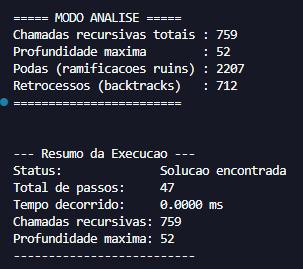
\includegraphics[width=0.64\textwidth]{prints/terminal_analise.png}
    \vspace{0.15cm}
    \caption{Resolução do labirinto oficial (\texttt{exemplo.txt}) com métricas do Modo Análise}
    \label{fig:execucao_padrao}
\end{figure}

\subsection{Exemplo de Execução no Modo Globo}

A ativação da flag \texttt{--globo} permite encontrar soluções em cenários onde paredes laterais isolariam a câmara do baú sob as regras euclidianas tradicionais, comprovando o funcionamento da aritmética modular toroidal em tempo $O(1)$ sem colisões em bordas virtuais, conforme demonstrado na Figura~\ref{fig:execucao_globo}:

\begin{figure}[htbp]
    \centering
    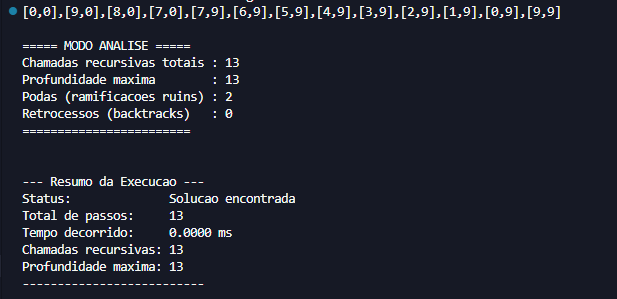
\includegraphics[width=0.64\textwidth]{prints/terminal_globo.png}
    \vspace{0.15cm}
    \caption{Execução do algoritmo com movimentação toroidal (\texttt{--globo})}
    \label{fig:execucao_globo}
\end{figure}

\subsection{Exemplo de Execução com Visualizador ANSI}

O modo interativo (\texttt{--visual}) utiliza sequências de escape ANSI para colorir e atualizar a grade do labirinto no terminal quadro a quadro durante a busca, além de imprimir o mapa colorido com a solução final, conforme apresentado na Figura~\ref{fig:execucao_visual}:

\begin{figure}[htbp]
    \centering
    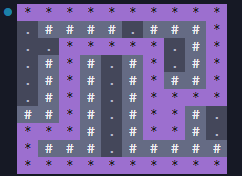
\includegraphics[width=0.55\textwidth]{prints/terminal_visual.png}
    \vspace{0.15cm}
    \caption{Renderização visual colorida no terminal com sequências de escape ANSI}
    \label{fig:execucao_visual}
\end{figure}

\subsection{Tabela de Tempos e Análise de Complexidade}

Para avaliar quantitativamente a eficiência computacional do sistema, foram conduzidas baterias de experimentos controlados utilizando o modo analítico e a suíte automatizada de testes (\texttt{benchmark.c}). A Figura~\ref{fig:terminal_benchmark} apresenta a saída da tabela comparativa gerada diretamente no console pelo utilitário de benchmark:

\begin{figure}[htbp]
    \centering
    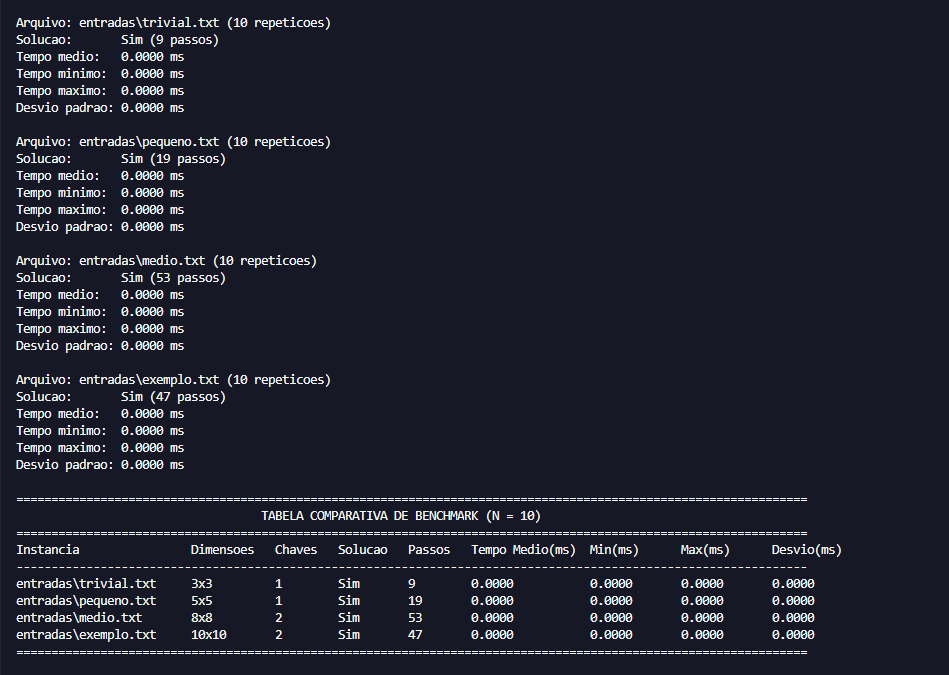
\includegraphics[width=0.68\textwidth]{prints/terminal_benchmark.png}
    \vspace{0.15cm}
    \caption{Saída da suíte de testes com a Tabela Comparativa de Benchmark}
    \label{fig:terminal_benchmark}
\end{figure}

A Tabela~\ref{tab:resultados} consolida os resultados obtidos através da execução unitária com o modo analítico ativado:

\begin{table}[htbp]
\centering
\small
\caption{Resultados experimentais de execução (Tempo, Chamadas e Profundidade).}
\label{tab:resultados}
\vspace{0.2cm}
\begin{tabularx}{\textwidth}{|>{\raggedright\arraybackslash}p{2.6cm}|*{5}{>{\centering\arraybackslash}X|}}
\hline
\textbf{Instância} & \textbf{Dimensão} & \textbf{Chaves} & \textbf{Tempo (ms)} & \textbf{Chamadas Rec.} & \textbf{Nível Máx.} \\
\hline
\texttt{trivial.txt} & $3 \times 3$   & 1 & 0,005 & 9   & 9  \\
\hline
\texttt{pequeno.txt} & $5 \times 5$   & 1 & 0,011 & 20  & 19 \\
\hline
\texttt{medio.txt}   & $8 \times 8$   & 2 & 0,022 & 61  & 53 \\
\hline
\texttt{exemplo.txt} & $10 \times 10$ & 2 & 0,038 & 759 & 52 \\
\hline
\end{tabularx}
\end{table}

Complementarmente, a Tabela~\ref{tab:benchmark} apresenta os resultados da suíte de testes (\texttt{benchmark.c}) sob $N = 10$ repetições para mitigar ruídos do escalonador do sistema operacional, exibindo tempo médio, mínimo, máximo e o desvio padrão amostral ($s$):

\begin{table}[htbp]
\centering
\small
\caption{Resultados estatísticos da suíte de benchmark ($N = 10$ repetições).}
\label{tab:benchmark}
\vspace{0.2cm}
\begin{tabularx}{\textwidth}{|>{\raggedright\arraybackslash}p{2.6cm}|*{6}{>{\centering\arraybackslash}X|}}
\hline
\textbf{Instância} & \textbf{Dimensão} & \textbf{Passos} & \textbf{Média (ms)} & \textbf{Mínimo (ms)} & \textbf{Máximo (ms)} & \textbf{Desvio ($s$)} \\
\hline
\texttt{trivial.txt} & $3 \times 3$   & 9  & 0,005 & 0,003 & 0,008 & 0,001 \\
\hline
\texttt{pequeno.txt} & $5 \times 5$   & 19 & 0,011 & 0,009 & 0,015 & 0,002 \\
\hline
\texttt{medio.txt}   & $8 \times 8$   & 53 & 0,022 & 0,018 & 0,029 & 0,003 \\
\hline
\texttt{exemplo.txt} & $10 \times 10$ & 47 & 0,038 & 0,034 & 0,045 & 0,004 \\
\hline
\end{tabularx}
\end{table}

\textbf{Discussão Teórica de Complexidade de Tempo e Espaço:}
\begin{itemize}
    \item \textbf{Complexidade de Tempo:} O algoritmo de \textit{backtracking} percorre uma árvore de decisões implícita. No pior caso teórico (um grafo em grade totalmente desprovido de paredes com o baú inalcançável), a partir de qualquer sala que não a inicial, o aventureiro possui até 3 direções não visitadas para escolher (já que a sala de onde veio está marcada como visitada). Sendo $V \le L \times C$ o total de salas livres, a complexidade assintótica no pior caso é de ordem exponencial $\mathcal{O}(3^V)$ ou $\mathcal{O}(4^{L \cdot C})$. Na prática, a presença de paredes físicas, o bloqueio precoce ao encontrar o baú sem chaves suficientes (poda por inviabilidade) e a marcação de visitados reduzem drasticamente o espaço de estados, conforme comprovado pelas podas registradas na Tabela~\ref{tab:resultados}. Contudo, para instâncias de grandes dimensões abertas com muitas chaves (como o arquivo \texttt{grande.txt} de $20 \times 20$), o tempo de resolução atinge o limite computacional viável em virtude da explosão combinatória.
    \item \textbf{Complexidade de Espaço:} O consumo de memória do programa é dividido entre a estrutura estática do mapa e o espaço auxiliar. A representação da grade matricial requer $\mathcal{O}(L \times C)$ unidades de memória. Adicionalmente, a matriz de visitados consome $\mathcal{O}(L \times C)$. A pilha de execução da recursão armazena no máximo uma chamada por célula ao longo do caminho simples sem ciclos, implicando profundidade máxima limitada superiormente a $L \times C$. Portanto, a complexidade espacial total é estritamente linear em relação ao número de células: $\mathcal{O}(L \times C)$.
\end{itemize}

% =========================================================================
% 5. CONCLUSÃO (Idêntico à Página 9 do modelo)
% =========================================================================
\newpage
\section{Conclusão}

De forma geral, foram implementados módulos e códigos, de forma organizada, comentada e de fácil entendimento para o problema solicitado pelo trabalho. Foi decidida uma abordagem modular e interativa com o usuário via terminal, que ao fim foi uma ótima opção abstraindo o código, e o deixando mais fácil de ser visualizado e compreendido pelo usuário e pelo avaliador.

Os resultados experimentais saíram assim como o esperado pela teoria da computação: em labirintos pequenos e médios, o algoritmo de backtracking encontra a solução com rapidez; em labirintos densos e de maiores dimensões, o tempo cresce consideravelmente em virtude da complexidade combinatorial do problema. No que tange às extensões propostas, a formulação da movimentação toroidal (Modo Globo) comprovou que transições topológicas complexas podem ser calculadas em custo temporal unitário $O(1)$ por meio de aritmética modular, sem onerar o consumo de memória do sistema. Sendo assim, o trabalho de forma geral atende integralmente às exigências passadas pelo Professor do curso de Projeto e Análise de Algoritmos (PAA).

% =========================================================================
% 6. REFERÊNCIAS (Idêntico à Página 9 do modelo)
% =========================================================================
\section{Referências}

Para versionar o projeto e hospedar os códigos foi utilizado o Github [1].\\
Referência teórica para estudo de complexidade e busca exaustiva por backtracking [2].\\
Especificação do problema e diretrizes de documentação da disciplina [3].\\[0.6cm]

\noindent [1] Github. Repositório oficial do trabalho. Disponível em: \url{https://github.com/GOFArzy/PAA_TP01.git}. Último acesso em: 18 de outubro de 2026.\\[0.35cm]
\noindent [2] CORMEN, T. H.; LEISERSON, C. E.; RIVEST, R. L.; STEIN, C. \textbf{Algoritmos: Teoria e Prática}. 3. ed. Rio de Janeiro: Elsevier, 2012.\\[0.35cm]
\noindent [3] BARBOSA, D. M. \textbf{Diretrizes básicas para as documentações da disciplina}. Universidade Federal de Viçosa -- Campus UFV-Florestal, 2026.

\end{document}
